\documentclass[aspectratio=169,10pt]{beamer}

\usepackage[T1]{fontenc}
\usepackage{lmodern}
\usepackage{graphicx}
\usepackage{booktabs}
\usepackage{array}
\usepackage{tikz}
\usetikzlibrary{arrows.meta,positioning}

% ---------------------------------------------------------------- style
\definecolor{ink}{HTML}{1F2937}
\definecolor{muted}{HTML}{6B7280}
\definecolor{sun}{HTML}{D97706}
\definecolor{sky}{HTML}{2563EB}
\definecolor{good}{HTML}{15803D}
\definecolor{bad}{HTML}{B91C1C}
\definecolor{panel}{HTML}{E5E7EB}

\usetheme{default}
\setbeamertemplate{navigation symbols}{}
\setbeamercolor{normal text}{fg=ink}
\setbeamercolor{frametitle}{fg=ink}
\setbeamercolor{structure}{fg=sun}
\setbeamercolor{itemize item}{fg=sun}
\setbeamercolor{itemize subitem}{fg=muted}
\setbeamerfont{frametitle}{series=\bfseries,size=\Large}
\setbeamertemplate{itemize item}{\raisebox{0.15em}{\scalebox{0.7}{$\blacksquare$}}}
\setbeamertemplate{itemize subitem}{--}
\setbeamertemplate{frametitle}{%
  \vspace{0.6em}\insertframetitle\par
  \vspace{-0.35em}{\color{sun}\rule{2.2em}{2pt}}\vspace{-0.2em}}
\setbeamertemplate{footline}{%
  \hfill{\color{muted}\scriptsize Solar Plant Manager \quad\insertframenumber\,/\,\inserttotalframenumber}\hspace{1.2em}\vspace{0.8em}}

\newcommand{\shot}[2][]{{\setlength{\fboxsep}{0pt}\color{panel}\fbox{\includegraphics[#1]{#2}}}}
\newcommand{\hl}[1]{{\color{sun}\textbf{#1}}}
\newcommand{\faint}[1]{{\color{muted}\small #1}}
\newcommand{\bignum}[2]{\begin{minipage}[t]{0.23\textwidth}\centering
  {\color{sun}\fontsize{22}{24}\selectfont\bfseries #1}\\[0.3em]{\color{muted}\footnotesize #2}\end{minipage}}

\tikzset{
  box/.style={draw=#1, fill=#1!8, rounded corners=3pt, align=center,
              font=\scriptsize, inner sep=5pt, text width=2.55cm, minimum height=1.5cm},
  box/.default=sky,
  flow/.style={-{Stealth[length=2.2mm]}, thick, color=muted},
}

\graphicspath{{screenshots/}{figures/}{../webapp/backend/analysis/figures/}}

\begin{document}

% ================================================================ 1 title
{\setbeamertemplate{footline}{}
\begin{frame}
  \vspace{2.2em}
  {\color{sun}\rule{3em}{3pt}}\\[0.8em]
  {\fontsize{30}{34}\selectfont\bfseries Solar Plant Manager}\\[0.5em]
  {\Large\color{muted} Monitoring, forecasting and fault detection for small solar plants}\\[2.6em]
  \textbf{Harsh Chattar} {\color{muted}22CS30028}\\[0.2em]
  \textbf{Abhinav Kumar Singh} {\color{muted}22CS30005}\\[1.2em]
  {\color{muted}Data Analytics 2026}
\end{frame}}

% ================================================================ 2 product
\begin{frame}{What we built}
  \begin{columns}[T]
    \column{0.40\textwidth}
    A day-to-day manager for a small plant's owner:
    \begin{itemize}\small\setlength\itemsep{0.45em}
      \item \textbf{Overview}: power now vs expected, energy, earnings, CO\textsubscript{2}, performance ratio
      \item \textbf{Production}: daily and monthly yield, inverter comparison
      \item \textbf{Forecast}: next 7 days, with measured accuracy
      \item \textbf{Health}: live fault detection, alerts, where energy is lost
      \item \textbf{Finance}: projected year, payback
    \end{itemize}
    \vspace{0.3em}
    \faint{Sign up, describe the plant, pair its gateway with a code; updates live.}
    \column{0.58\textwidth}
    \vspace{0.1em}
    \shot[width=\linewidth]{v2_overview_crop.png}
  \end{columns}
\end{frame}

% ================================================================ 3 architecture + data
\begin{frame}{How it works}
  \centering
  \vspace{0.2em}
  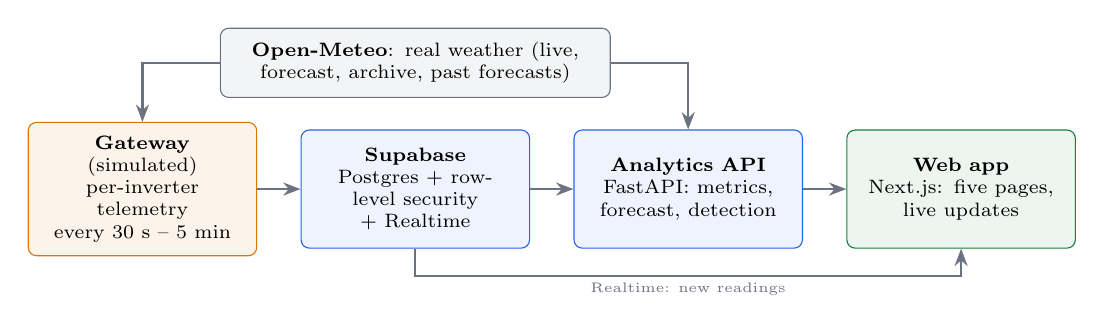
\begin{tikzpicture}[node distance=0.55cm, every node/.append style={minimum height=1.2cm}]
    \node[box=sun] (g) {\textbf{Gateway}\\(simulated)\\per-inverter telemetry\\every 30 s -- 5 min};
    \node[box=sky, right=of g] (db) {\textbf{Supabase}\\Postgres + row-level security\\+ Realtime};
    \node[box=sky, right=of db] (api) {\textbf{Analytics API}\\FastAPI: metrics,\\forecast, detection};
    \node[box=good, right=of api] (app) {\textbf{Web app}\\Next.js: five pages,\\live updates};
    \node[box=muted, above=0.4cm of db, text width=4.6cm, minimum height=0.7cm] (om)
      {\textbf{Open-Meteo}: real weather (live, forecast, archive, past forecasts)};
    \draw[flow] (g) -- (db); \draw[flow] (db) -- (api); \draw[flow] (api) -- (app);
    \draw[flow] (db.south) -- ++(0,-0.35) -| node[pos=0.25, below, font=\tiny, color=muted, minimum height=0pt, inner sep=2pt] {Realtime: new readings} (app.south);
    \draw[flow] (om.west) -| (g.north);
    \draw[flow] (om.east) -| (api.north);
  \end{tikzpicture}
  \vspace{0.6em}
  \begin{columns}[T]
    \column{0.49\textwidth}
    \textbf{The data}
    \begin{itemize}\footnotesize\setlength\itemsep{0.15em}
      \item \textbf{Inverters are simulated} (no hardware): \textbf{real weather} $\rightarrow$ pvlib physics (sun angle, tilt, heat, ageing)
      \item Real-life mess added: 3\% sensor noise, $\pm$6\% sky error, shading, faults of 5--40\% for 2--8 h
      \item Every fault is logged: \hl{an answer key to measure detection}
    \end{itemize}
    \column{0.47\textwidth}
    \textbf{The system}
    \begin{itemize}\footnotesize\setlength\itemsep{0.15em}
      \item The gateway pairs with a code and holds its own device token, like a real data logger
      \item The API reads data \emph{as the signed-in user}: no admin keys
    \end{itemize}
  \end{columns}
\end{frame}

% ================================================================ 5 metrics
\begin{frame}{Plant metrics}
  \begin{columns}[T]
    \column{0.42\textwidth}
    \begin{itemize}\small\setlength\itemsep{0.45em}
      \item \textbf{Performance ratio} (IEC 61724) = energy $\div$ (sunlight on panels $\times$ kWp). Healthy: 75--85\%; test plant: 86\% (30 d)
      \item \textbf{Specific yield} = kWh per installed kWp, to compare plants of any size
      \item \textbf{Availability}, earnings, CO\textsubscript{2} avoided (0.716 kg/kWh, Indian grid)
      \item \textbf{Loss breakdown}: sunlight potential $\rightarrow$ heat $\rightarrow$ ageing $\rightarrow$ inverter $\rightarrow$ downtime $\rightarrow$ faults $\rightarrow$ delivered (adds up exactly)
      \item \textbf{Payback}: a typical year of real weather at the site: 13.8 MWh, 5.6 years on 3.5 lakh
    \end{itemize}
    \column{0.56\textwidth}
    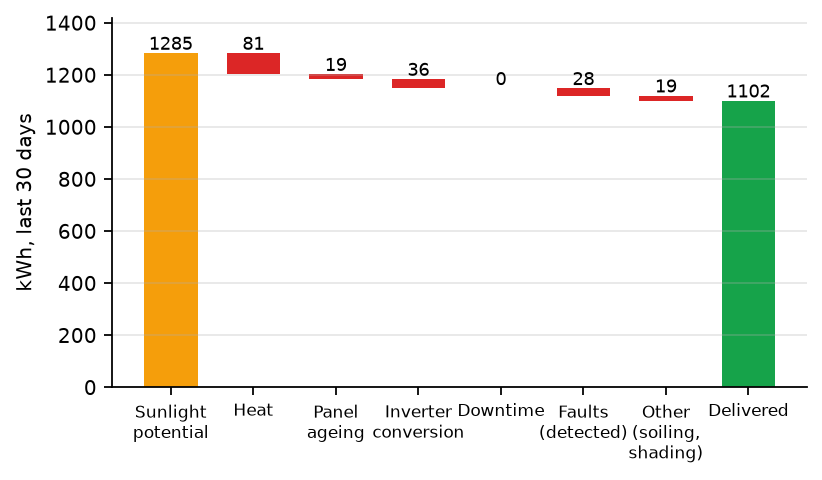
\includegraphics[width=\linewidth]{losses.png}\\[0.2em]
    \faint{Where the test plant's energy went, last 30 days (Health page).}
  \end{columns}
\end{frame}

% ================================================================ 6 forecast
\begin{frame}{Forecasting: does it beat the naive guess?}
  \begin{columns}[T]
    \column{0.46\textwidth}
    \small
    Weather forecast $\rightarrow$ physics $\rightarrow$ $\times$ plant calibration (actual $\div$ physics, last 14 days).
    Scored against the forecast \emph{as issued the day before}.
    \vspace{0.6em}

    \footnotesize
    \renewcommand{\arraystretch}{1.2}
    \begin{tabular}{@{}lrr@{}}
      \toprule
      12 months, Pune & Error (kWh/day) & Forecast is \\
      \midrule
      \textbf{Day-ahead forecast} & \textbf{1.54} (4.6\%) & \\
      Same as yesterday & 2.65 & \textbf{42\% better} \\
      30-day average & 3.72 & \textbf{59\% better} \\
      \midrule
      Monsoon (Jun--Sep) & 2.77 (8.9\%) & 34\% better \\
      \bottomrule
    \end{tabular}\\[0.5em]
    \faint{In the app: the last 7 days' accuracy ($\pm$5.7\%), 35\% better than ``same as yesterday''.}
    \column{0.52\textwidth}
    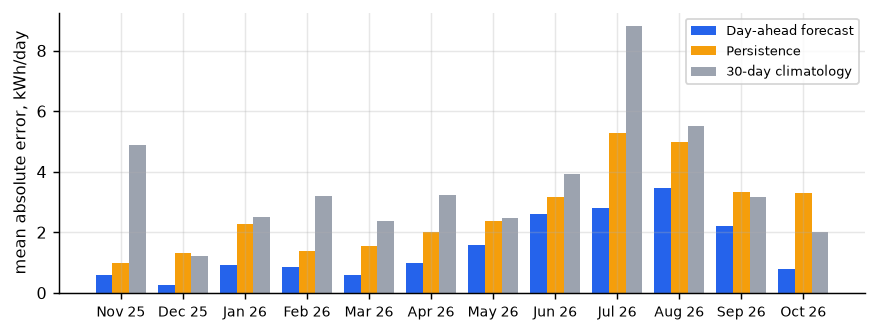
\includegraphics[width=\linewidth]{forecast_mae_by_month.png}\\[0.3em]
    \faint{Ahead of both naive methods in every month; the monsoon triples the error.}
  \end{columns}
\end{frame}

% ================================================================ 7 detection method
\begin{frame}{Fault detection}
  \begin{columns}[T]
    \column{0.42\textwidth}
    \small
    \textbf{Learn what healthy output looks like, flag the shortfall}
    \begin{itemize}\setlength\itemsep{0.3em}
      \item Expected power from weather + \textbf{the median of the other inverters}
      \item Shortfall = (expected $-$ actual) $\div$ expected, smoothed
      \item Threshold = median + 2.5 robust $\sigma$ of held-out residuals: \hl{never uses the labels}
    \end{itemize}
    \textbf{Four detectors compared}: physics baseline, Random Forest, Gradient Boosting, Isolation Forest (unsupervised)\\[0.4em]
    \faint{Live: a 30\% fault injected on the gateway is flagged within 1--3 minutes.}
    \column{0.56\textwidth}
    \shot[width=\linewidth]{v2_health_crop.png}
  \end{columns}
\end{frame}

% ================================================================ 8 which model
\begin{frame}{Which detector? Only some differences are real}
  \begin{columns}[T]
    \column{0.52\textwidth}
    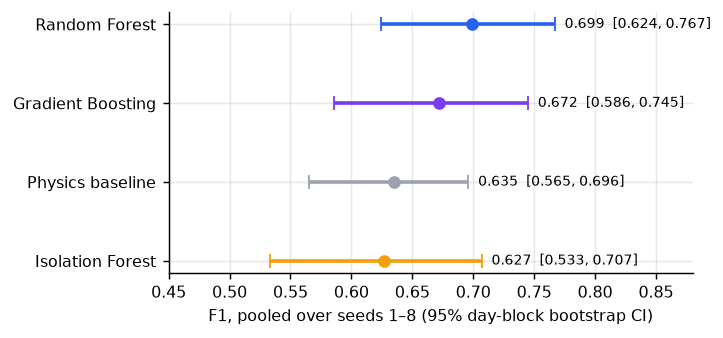
\includegraphics[width=\linewidth]{f1_ci.png}\\[0.2em]
    \faint{F1 pooled over 8 seeds; 95\% CI by day-block bootstrap.}
    \column{0.45\textwidth}
    \small
    \begin{itemize}\setlength\itemsep{0.45em}
      \item Random Forest \textbf{beats} the physics baseline (+0.065, CI +0.007 to +0.124) and Isolation Forest
      \item Random Forest vs Gradient Boosting: \textbf{tied} (CI crosses 0)
      \item Per episode, a trade-off per-hour F1 hid:
    \end{itemize}
    \vspace{0.2em}
    \scriptsize
    \renewcommand{\arraystretch}{1.15}
    \begin{tabular}{@{}lcc@{}}
      \toprule
      & Episodes caught & Alarms that are real \\
      \midrule
      Random Forest & 68\% & 65\% \\
      Gradient Boosting & 60\% & 72\% \\
      Physics baseline & \textbf{84\%} & 35\% \\
      \bottomrule
    \end{tabular}
  \end{columns}
\end{frame}

% ================================================================ 9 limits
\begin{frame}{Detection limit, and what makes the ML worth it}
  \centering
  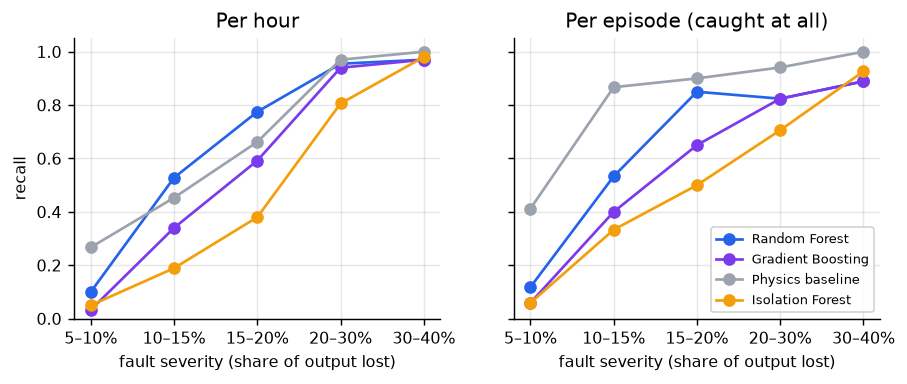
\includegraphics[width=0.49\textwidth]{recall_by_severity.png}\hfill
  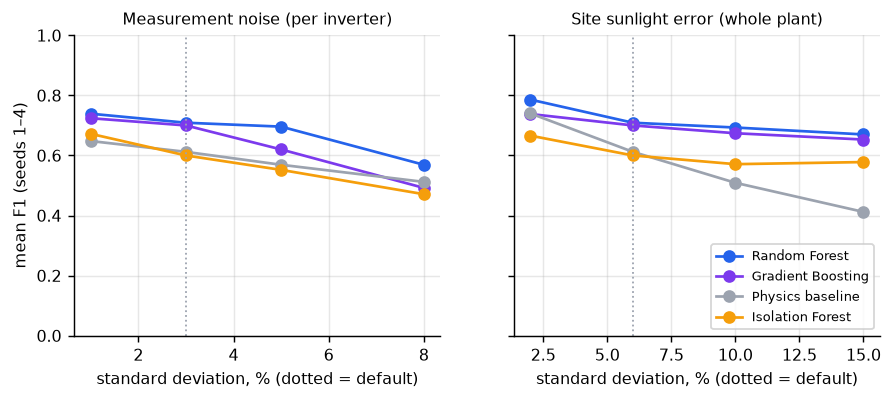
\includegraphics[width=0.49\textwidth]{sensitivity_noise.png}\\[0.4em]
  \raggedright
  \begin{itemize}\small\setlength\itemsep{0.3em}
    \item \textbf{The limit as a curve}: Random Forest catches 10\% of hours at 5--10\% loss, 53\% at 10--15\%, 96\%+ above 20\%. Mild faults hide in normal noise.
    \item \textbf{Sky error separates the methods}: as the plant-wide sunlight error grows 2\% $\rightarrow$ 15\%, the physics rule falls 0.74 $\rightarrow$ 0.41 F1; Random Forest only 0.79 $\rightarrow$ 0.67.
    \item \textbf{Why}: the Random Forest is effectively a \hl{peer comparison}. Shuffling the neighbours' output drops R\textsuperscript{2} by 1.5; any weather input by $<$0.02. Neighbours share the sky error, so it cancels. Blind spot: a fault hitting \emph{every} inverter at once.
  \end{itemize}
\end{frame}

% ================================================================ 11 limitations
\begin{frame}{Limitations and next steps}
  \begin{columns}[T]
    \column{0.47\textwidth}
    \textbf{Limitations}
    \begin{itemize}\small\setlength\itemsep{0.4em}
      \item Inverter output is simulated; detection numbers describe this simulator (and we showed how they move with it)
      \item Benchmark: one month, one site; the forecast study covers a full year
      \item Forecast ``actual'' is reanalysis weather, not an on-site sensor
      \item Model settings tuned on the seeds they're scored on (mild optimism)
    \end{itemize}
    \column{0.47\textwidth}
    \textbf{Next}
    \begin{itemize}\small\setlength\itemsep{0.4em}
      \item Real data in: CSV import from an inverter portal, then real hardware
      \item Peer comparison + weather check as the detector (F1 0.78 in experiments)
      \item Soiling and cleaning advice; email alerts
      \item Deployment
    \end{itemize}
  \end{columns}
\end{frame}

% ================================================================ 12 takeaways
\begin{frame}{Takeaways}
  \vspace{0.8em}
  \centering
  \bignum{42\%}{lower forecast error\\than ``same as yesterday''}\hfill
  \bignum{0.70}{F1 fault detection\\(CI 0.62--0.77)}\hfill
  \bignum{$>$20\%}{faults caught\\$\sim$96\% of the time}\hfill
  \bignum{5.6 yr}{payback, from a\\typical year of weather}\\[1.8em]
  \raggedright
  \begin{itemize}\setlength\itemsep{0.5em}
    \item A working plant manager: live monitoring, metrics, forecasts, health and finance on one plant's own data
    \item Simulated faults on real weather made detection \emph{measurable}; bootstrap CIs show which differences are real
    \item ML earns its place where the weather data can't be trusted: comparing inverters with each other
  \end{itemize}
  \vspace{1em}
  \centering{\Large\bfseries Thank you}\quad{\color{muted}Questions?}
\end{frame}

\end{document}
